\section{Requisiti funzionali}

Un'azienda dispone di un server su cui ha installato il virtualizzatore VMware che permette di creare/gestire macchine virtuali. Una macchina virtuale ha le stesse funzionalità di un computer fisico ma utilizza componenti hardware astratte. L'azienda ne vuole utilizzare una per esporre dei servizi su internet. Per farlo si serve un router che ha due schede di rete, una con indirizzo IP pubblico 79.61.138.204 e l'altra con IP privato 10.222.111.1 che si affaccia sulla LAN 10.222.111.0/24.
L'ambiente è composto da una prima macchina virtuale chiamata vm firewall su cui gira il sistema operativo CentOS 7, una distribuzione linux. La macchina dispone di un'unica scheda di rete (escludendo l'interfaccia di loopback) la ens160, corrispondente all'indirizzo IP 10.222.111.2.
Le risorse assegnate alla vm sono:
\begin{itemize}
    \item  8 core
    \item  32 GB ram
    \item 250 GB hdd
\end{itemize}

Il router è configurato in modo da inoltrare tutti i pacchetti che hanno come destinatario 79.61.138.204 sull'interfaccia ens160 della vm firewall.

L'azienda ha l'esigenza di utilizzare dei servizi non recenti, non sempre aggiornati e teme per la sicurezza della propria rete. Il suo obiettivo è garantire riservatezza, integrità, disponibilità dei dati in qualsiasi momento. Se ad esempio non riuscisse a mantenere private le informazioni personali degli utenti che utilizzano i servizi offerti, andrebbe incontro a gravi ripercussioni (anche legali). Allo stesso modo, se non riuscisse a mantenere attivo il servizio a causa di malfunzionamenti potrebbe subire perdite economiche. Allo scopo di proteggere la rete vuole configurare manualmente il firewall con iptables.

I servizi che vuole esporre in rete sono:
\begin{itemize}
    \item  un web server usando il protocollo applicativo HTTP (sulla porta 80) e HTTPS (sulla porta 443) pubblicato utilizzando il servizio Http Apache versione 2.4.6
    \item un web server con Tomcat versione 7.0.76
    \item un file server con Samba versione 4.10.16
\end{itemize}

L'azienda richiede i seguenti requisiti funzionali, legati ancora una volta al tema della sicurezza.

\subsection{Requisito 1: monitoraggio del traffico}

Un utente deve essere in grado di utilizzare i servizi installati sulla macchina in sicurezza. Quando arriva del traffico sulle porte relative ai servizi installati, deve essere notificato e registrato, in modo che un amministratore di rete possa successivamente investigare il contenuto dei pacchetti se lo ritiene necessario. Deve essere possibile poter effettuare dei controlli mirati sui pacchetti, ad esempio analizzare solo le GET HTTP, solo i pacchetti provenienti da un IP o da un range di IP, su una porta o su un range di porte.

\subsection{Requisito 2: rilevazione di attacchi}

Devono poter essere rilevati possibili attacchi in rete. Se avviene una rilevazione deve essere notificata all'amministratore, in modo che possa intervenire per contrastarla. L'avviso deve essere chiaro e far riferimento all'attacco. Ad esempio un volume non indifferente di traffico rilevato in modo continuo deve essere identificato come ``possible DoS attack'' e non ``UDP packet detected'' o ``TCP packet detected''.

\subsection{Requisito 3: prevenzione di attacchi}

Devono essere prese delle misure contro possibili attacchi in rete. Non è sufficiente rilevare la minaccia, il sistema deve essere in grado di prevenire l'attacco in modo da da esonerare l'amministratore da un intervento repentino (qualora possibile). Si richiede quindi l'uso di una tecnologia capace di intervenire attivamente per eliminare pacchetti che sono ritenuti sospetti.

\begin{figure}[htb]
    \begin{center}
        \begin{tabular}{l}
            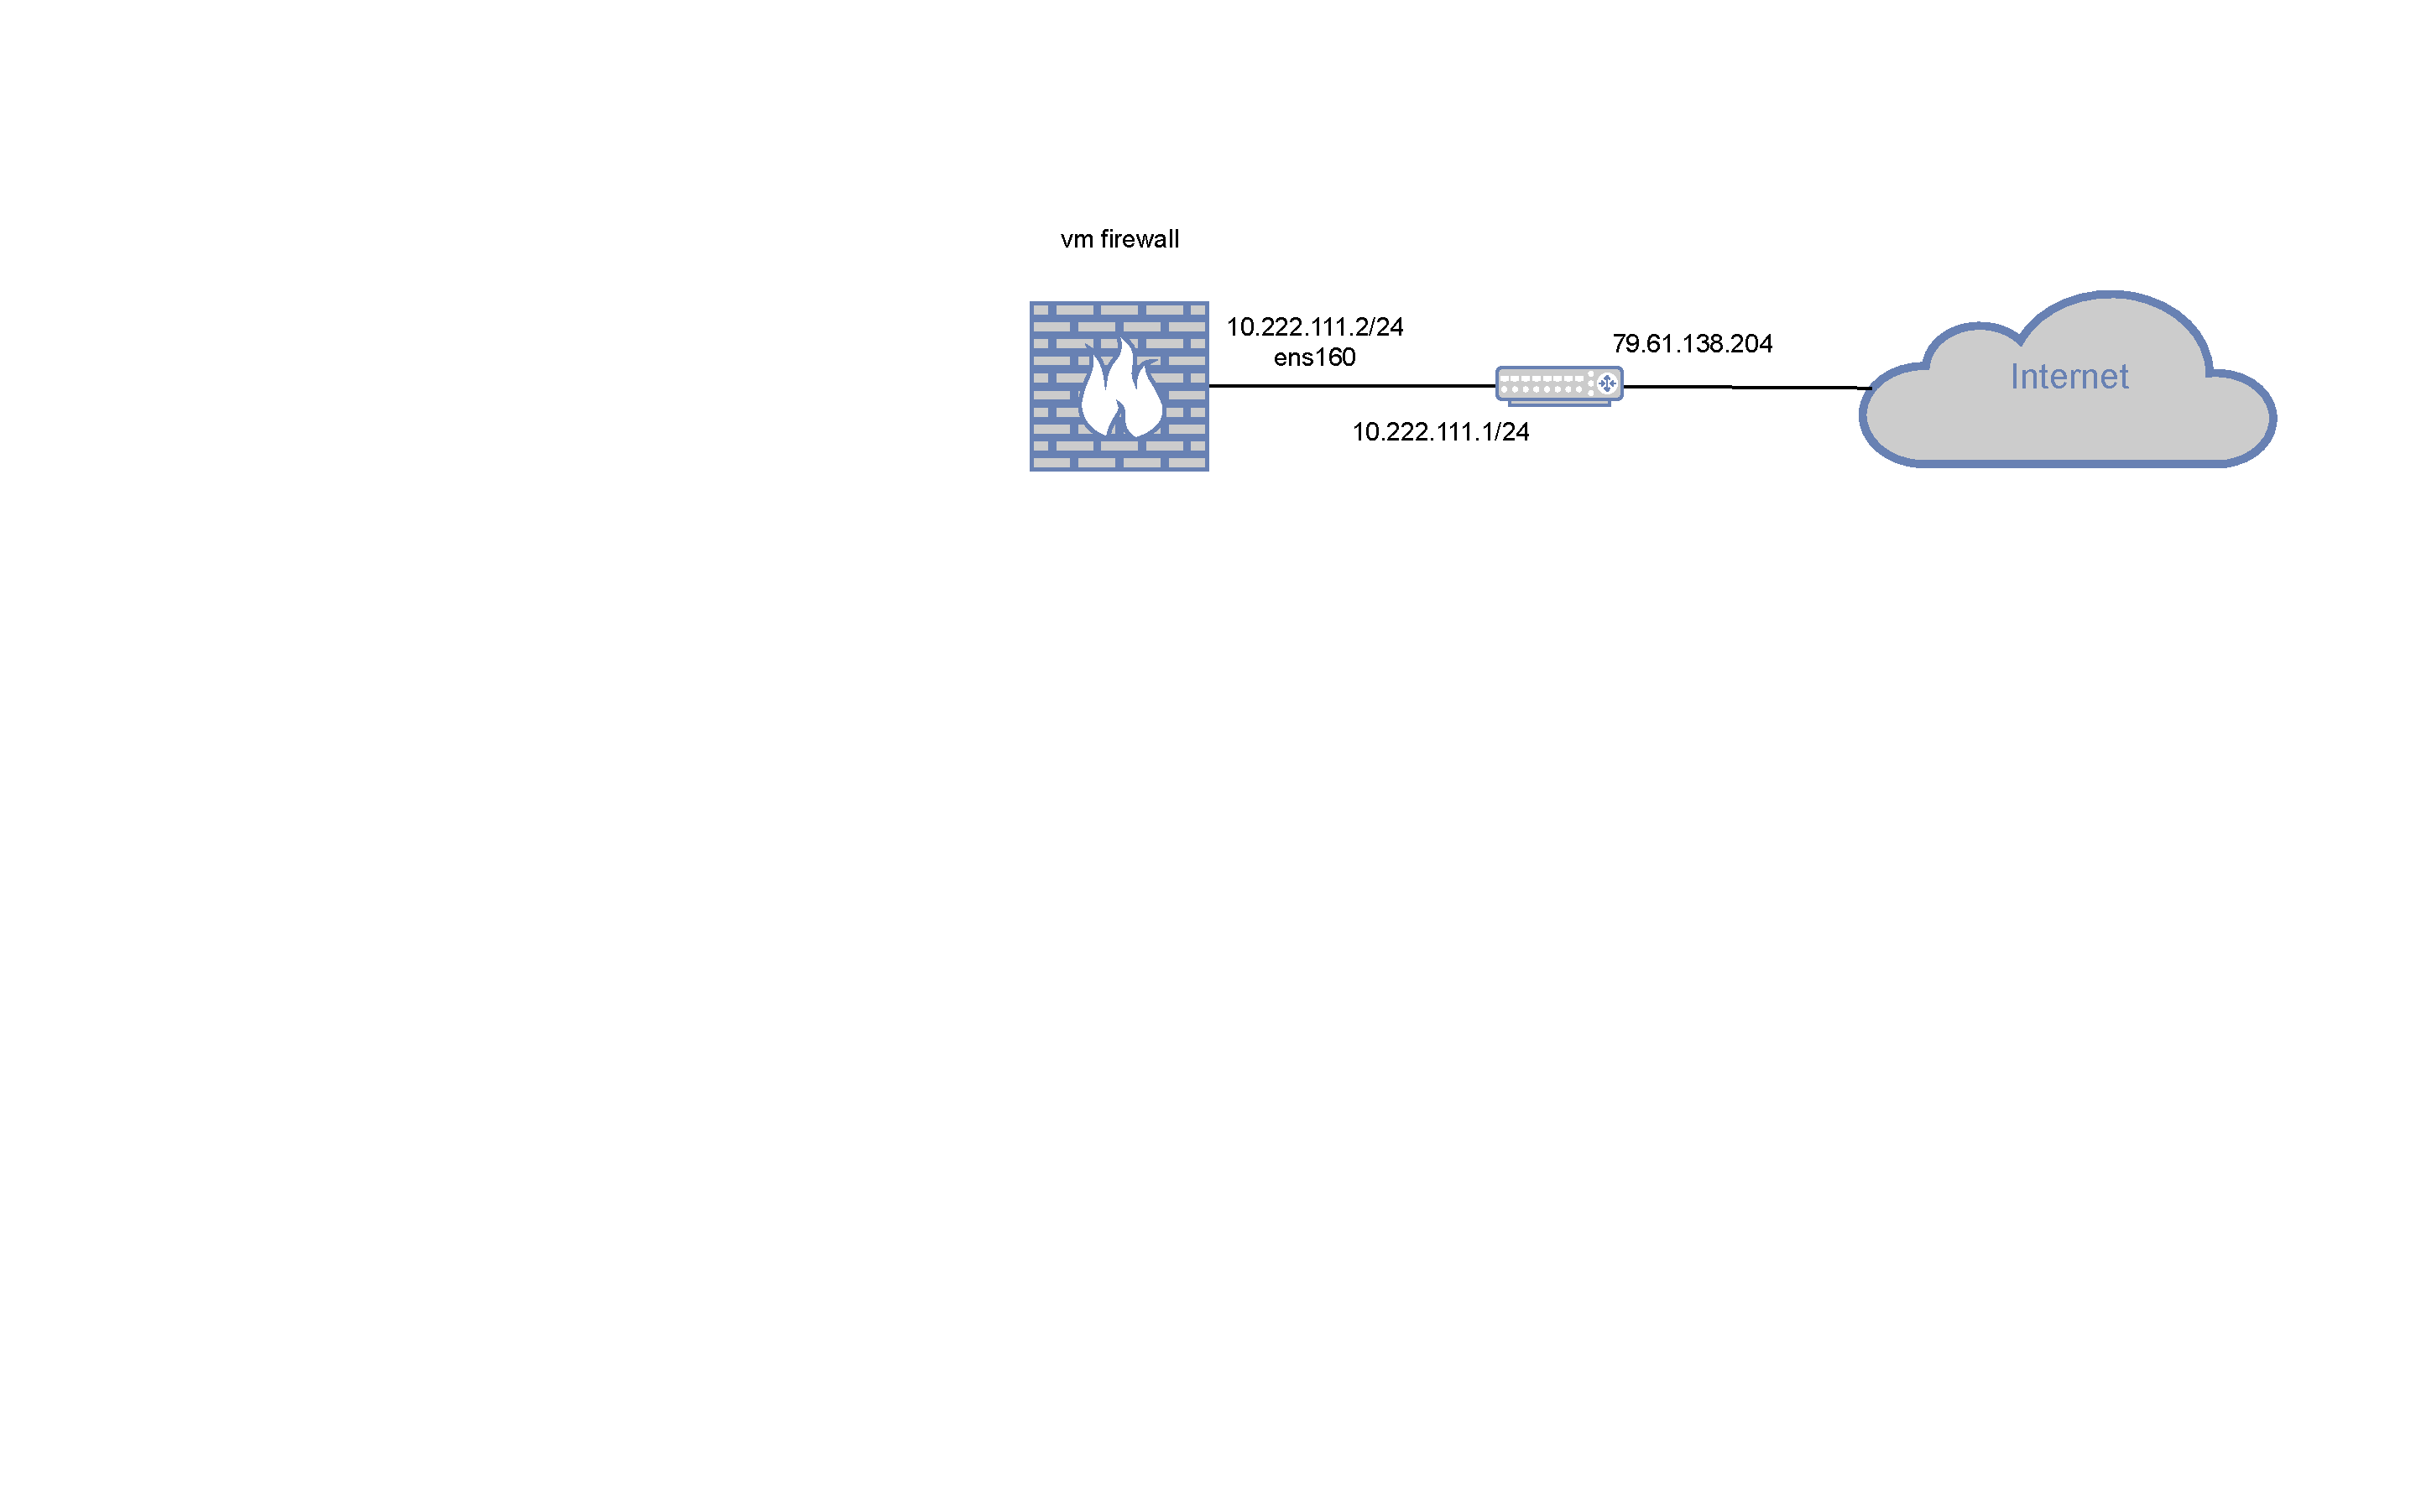
\includegraphics[width=15cm]{figure/net_requirement.pdf}
        \end{tabular}
    \end{center}
    \caption{Rete nel suo stato primordiale.}
\end{figure}

\section{Requisiti non funzionali}

L'azienda richiede anche che venga rispettata una serie di requisiti non funzionali.

\subsection{Modularità}

Un sistema modulare separa funzionalità distinte in aree distinte. Il vantaggio di un sistema di questo tipo è riuscire a identificare una correzione o riuscire ad apportare un cambiamento, senza dover stravolgere la configurazione precedente, individuando l'area interessata e intervenendo localmente. Le modifiche ricadranno esclusivamente su di essa e non si propagheranno sull'intero sistema.

\subsection{Scalabilità}

Un sistema scalabile permette l’aggiunta di funzionalità e ulteriori requisiti a posteriori senza stravolgerne la struttura, ma solo applicando le nuove caratteristiche richieste nell'area di competenza. Se ad esempio nel prossimo futuro l'azienda decidesse di espandersi e di esporre nuovi servizi, potrebbe farlo senza riorganizzare l'intera struttura della rete, agendo in un contesto molto più ristretto.

\subsection{Open source}

L'azienda richiede che vengano utilizzati software open source. Non solo perché non richiedono costi iniziali, ma perché garantiscono maggiore stabilità e protezione, grazie alla loro diffusione e al supporto di sviluppatori esperti che partecipano alla comunità. Un software di questo tipo libera l’azienda dal dipendere da un unico produttore, un’unica architettura, un unico protocollo, al contrario permette un alto livello di integrazione. Il codice open source è continuamente revisionato e corretto. Nel caso di sistemi di rilevazione e prevenzione delle intrusioni utilizzare codice affidabile e aggiornato garantisce di raggiungere un secondo obiettivo: avere un basso numero di falsi positivi e negativi.